%----------------------------------------------------------------------------------------
%	PACKAGES AND OTHER DOCUMENT CONFIGURATIONS
%----------------------------------------------------------------------------------------

\documentclass[paper=a4, fontsize=11pt]{scrartcl} % A4 paper and 11pt font size
\usepackage{graphicx} %For inserting pictures
\usepackage[T1]{fontenc} % Use 8-bit encoding that has 256 glyphs
\usepackage[english]{babel} % English language/hyphenation
\usepackage{amsmath,amsfonts,amsthm} % Math packages
\usepackage{float} %For H floats
%\allsectionsfont{\centering \normalfont\scshape} % Make all sections centered, the default font and small caps

\usepackage{fancyhdr} % Custom headers and footers
\pagestyle{fancyplain} % Makes all pages in the document conform to the custom headers and footers
\fancyhead{} % No page header - if you want one, create it in the same way as the footers below
\fancyfoot[L]{} % Empty left footer
\fancyfoot[C]{} % Empty center footer
\fancyfoot[R]{\thepage} % Page numbering for right footer
\renewcommand{\headrulewidth}{0pt} % Remove header underlines
\renewcommand{\footrulewidth}{0pt} % Remove footer underlines
\setlength{\headheight}{13.6pt} % Customize the height of the header

\numberwithin{equation}{section} % Number equations within sections (i.e. 1.1, 1.2, 2.1, 2.2 instead of 1, 2, 3, 4)
\numberwithin{figure}{section} % Number figures within sections (i.e. 1.1, 1.2, 2.1, 2.2 instead of 1, 2, 3, 4)
\numberwithin{table}{section} % Number tables within sections (i.e. 1.1, 1.2, 2.1, 2.2 instead of 1, 2, 3, 4)

\setlength\parindent{0pt} % Removes all indentation from paragraphs - comment this line for an assignment with lots of text
\DeclareGraphicsExtensions{.pdf,.png,.jpg}
\graphicspath{ {../images/} }
%----------------------------------------------------------------------------------------
%	TITLE SECTION
%----------------------------------------------------------------------------------------

\newcommand{\horrule}[1]{\rule{\linewidth}{#1}} % Create horizontal rule command with 1 argument of height

\title{	
\normalfont \normalsize 
\textsc{Dhirubhai Ambani Institute of Information and Communication Technology} \\ [25pt] % Your university, school and/or department name(s)
\horrule{0.5pt} \\[0.4cm] % Thin top horizontal rule
\huge Assignment 3 \\ % The assignment title
\horrule{2pt} \\[0.5cm] % Thick bottom horizontal rule
}

\author{Ganesh Iyer \\ 201311019 \\Developed using: Python(SimpleCV)}

\date{\normalsize\today} % Today's date or a custom date

\begin{document}

\maketitle % Print the title

%----------------------------------------------------------------------------------------
%	PROBLEM 1
%----------------------------------------------------------------------------------------

\section{Image Enhancement}
    \subsection{Enhancing scene image}
    In this problem we applied various contrast enhancement methods for improving the contrast of the given image.
        \begin{figure}[h!]
            \centering
            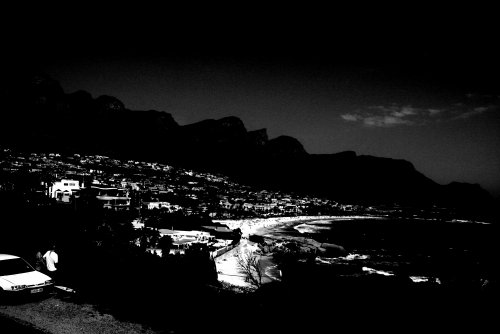
\includegraphics[clip,height=4cm]{scene}
            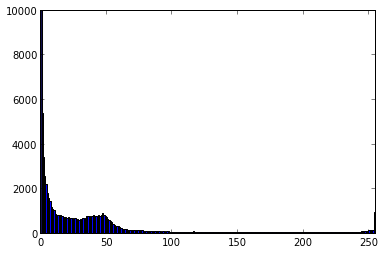
\includegraphics[clip,height=4cm]{scenehist}
            \caption{Original Image and corresponding histogram}
        \end{figure}

    From visually inspecting the image we realize that there is a very stark contrast in the image. We extracted the histogram of the image and from it we observe that there is a large concentration of pixels on the dark side. There is very little concentration in the middle of the histogram. Then near the higher intensities there is again a peak.

    We applied various techniques for enhancing the contrast of the image. Details of the same are reported below.
        \subsubsection{Log transformation}
        We applied the log transformation as our aim is to spread the darker gray levels in the image over a higher range. We applied a transformation of the form
        \\\(s = \frac{255}{log(1+255)} log(1+r)\)
        \begin{figure}[h!]
            \centering
            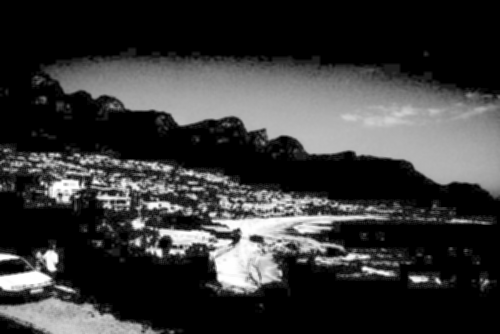
\includegraphics[clip,height=4cm]{logscene}
            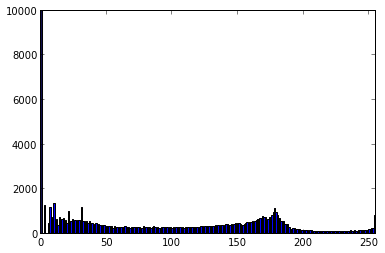
\includegraphics[clip,height=4cm]{logscenehist}

            \caption{Image and corresponding histogram obtained after applying log transformation and a gaussian blur with kernel size = 3}
        \end{figure}

        We obtain an image having much better contrast than the original image. We apply the gaussian blur to smoothen the image. It is evident from the histogram that there is a better distribution of the intensities in the transformed image. 
        \subsubsection{Powerlaw transfromation}
        The results from Log transformation encouraged us to experiment with powerlaw transformations(Gamma transfrorm) as its behaviour is similar to that of log transform when \(\gamma\) is fractional.
        \\\(s = 255r^\gamma \)

        We experimented with various vales of \(\gamma\) the results of which are reported.
        \begin{figure}[h!]
            \centering
            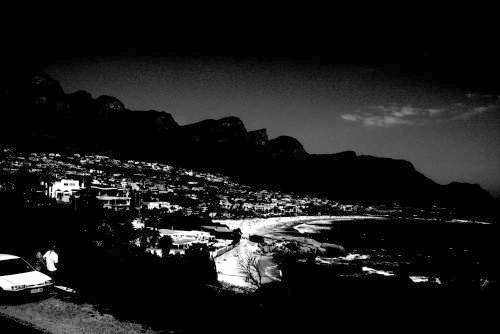
\includegraphics[clip,height=4cm]{gamma67}
            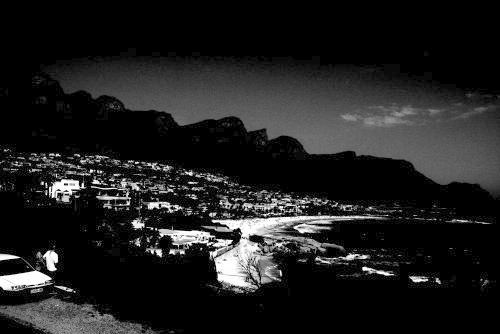
\includegraphics[clip,height=4cm]{gamma57}
            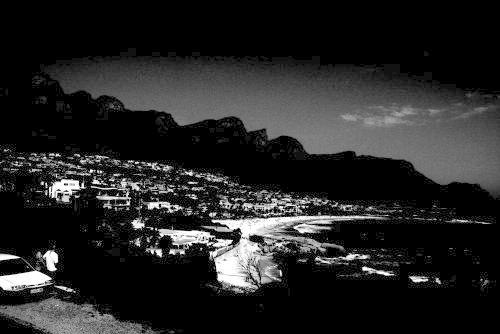
\includegraphics[clip,height=4cm]{gamma47}
            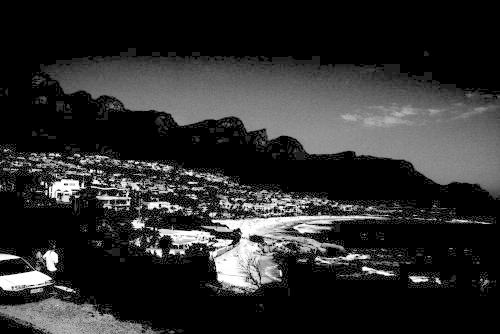
\includegraphics[clip,height=4cm]{gamma37}
            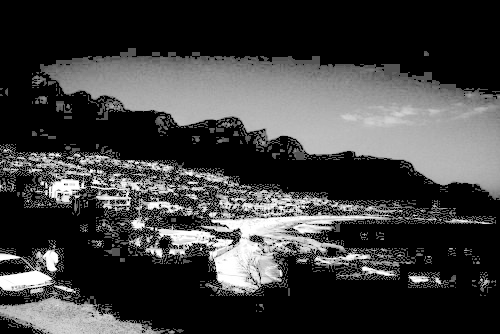
\includegraphics[clip,height=4cm]{gamma20}
            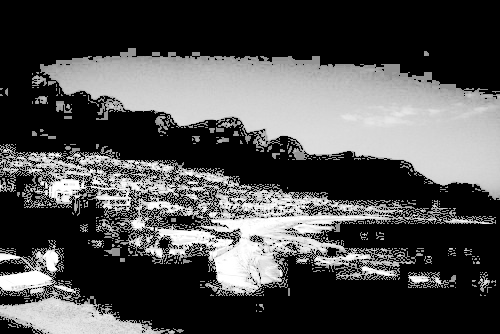
\includegraphics[clip,height=4cm]{gamma10}
            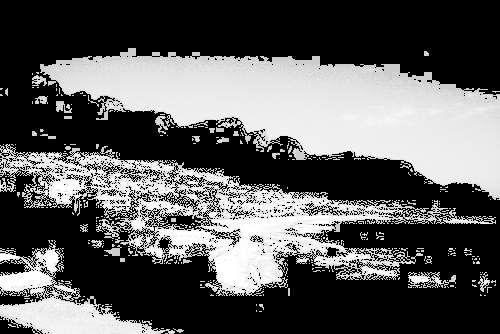
\includegraphics[clip,height=4cm]{gamma04}
            \caption{Images obtained by applying powerlaw transformation with values of \(\gamma = \{0.67,0.57, 0.47,0.37,0.20,0.10,0.04\}\)}
        \end{figure}
        From visually inspecting the images we find that the images obtained with \(\gamma\ \approx 0.37\) 
        \begin{figure}[h!]
            \centering
            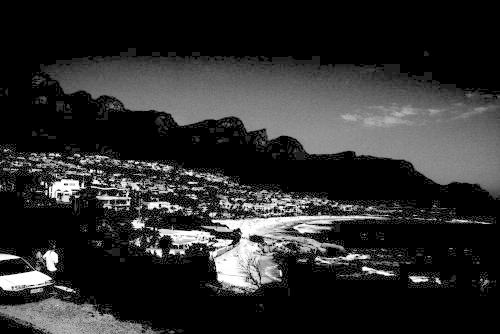
\includegraphics[clip,height=4cm]{gamma37}
            \caption{Images obtained by applying powerlaw transformation with value of \(\gamma = 0.37\) gave us the best results}
        \end{figure}
\subsection{Enhancing lctext.jpg}
    In the exercise we had to enhance the image shown in Fig ~\ref{fig:lctext}. We observe from the histogram that there is a uniformity at a global level. Hence global transformations will not have much of an effect.
        \begin{figure}[h!]
            \centering
            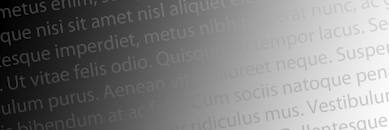
\includegraphics[clip,height=2cm]{lctext}
            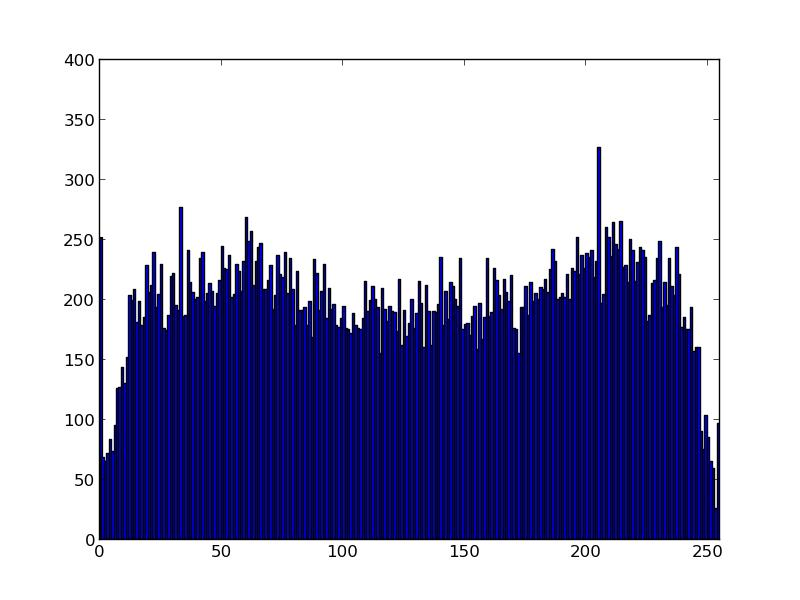
\includegraphics[clip,height=4cm]{lctexthist}
            \caption{Image and its histogram}
            \label{fig:lctext}
        \end{figure}
        In Fig ~\ref{fig:lctextlefthist} we analyse a section of the image we observe that the local histograms are not equalized. 
        \begin{figure}[h!]
            \centering
            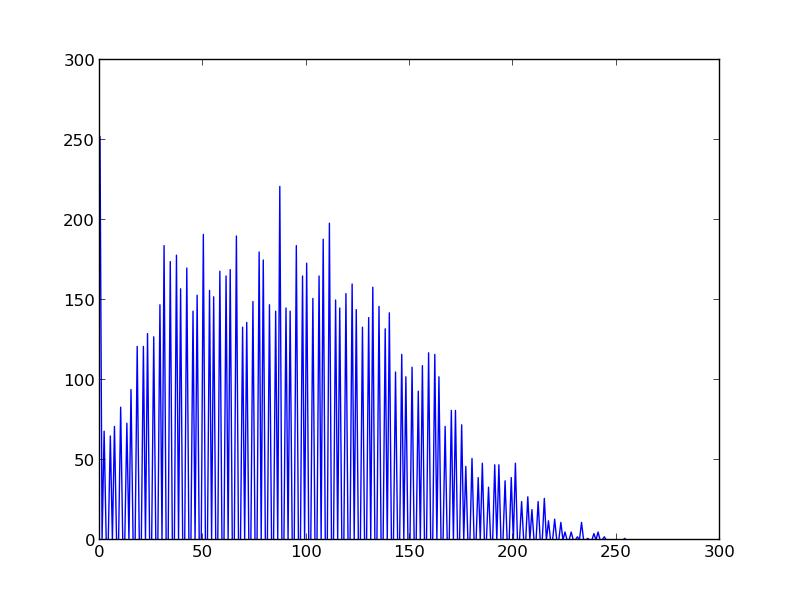
\includegraphics[clip,height=4cm]{lctextlefthist}
            \caption{Plot Histogram of \(100X100\) section of the image}
            \label{fig:lctextlefthist}
        \end{figure}

        Hence we apply local histogram equalization on a block size of \(8X8\) using the built-in function adapthisteq. The result is shown in Fig ~\ref{fig:lctextenhanced}
        \begin{figure}[h!]
            \centering
            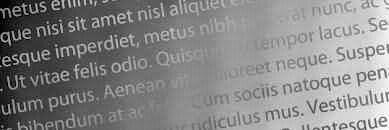
\includegraphics[clip,height=2cm]{lctextenhanced}
            \caption{Enhanced image after applying local histogram equalization}
            \label{fig:lctextenhanced}
        \end{figure}

\section{Exact histogram equalization}
adfssadf.
\end{document}
